%-------------------------
% Resume in LaTeX - Jake's Resume (Strict Single-Page Fit)
% Optimized for ATS & Fintech/AI Roles (e.g., Slice, Startups, Big Tech)
%------------------------

\documentclass[letterpaper,10pt]{article}

\usepackage{latexsym}
\usepackage[empty]{fullpage}
\usepackage{titlesec}
\usepackage{marvosym}
\usepackage[usenames,dvipsnames]{color}
\usepackage{verbatim}
\usepackage{enumitem}
\usepackage[hidelinks]{hyperref}
\usepackage{fancyhdr}
\usepackage[english]{babel}
\usepackage{tabularx}
\usepackage{graphicx}
\input{glyphtounicode}

% Clean, modern ATS font
\usepackage{charter}

\pagestyle{fancy}
\fancyhf{} 
\renewcommand{\headrulewidth}{0pt}
\renewcommand{\footrulewidth}{0pt}
\setlength{\footskip}{4.1pt} % Resolves fancyhdr footskip warning

% Margins calibrated for strict 1-page fit
\addtolength{\oddsidemargin}{-0.55in}
\addtolength{\evensidemargin}{-0.55in}
\addtolength{\textwidth}{1.1in}
\addtolength{\topmargin}{-0.6in}
\addtolength{\textheight}{1.2in}

\urlstyle{same}

\raggedbottom
\raggedright
\setlength{\tabcolsep}{0in}

% Section formatting
\titleformat{\section}{
  \vspace{-3pt}\scshape\raggedright\large
}{}{0em}{}[\color{black}\titlerule \vspace{-4pt}]

\pdfgentounicode=1

% Custom commands
\newcommand{\resumeItem}[1]{
  \item\small{
    {#1 \vspace{-2pt}}
  }
}

\newcommand{\resumeSubheading}[4]{
  \vspace{-2pt}\item
    \begin{tabular*}{0.98\textwidth}[t]{l@{\extracolsep{\fill}}r}
      \textbf{#1} & #2 \\
      \textit{\small#3} & \textit{\small #4} \\
    \end{tabular*}\vspace{-5pt}
}

\newcommand{\resumeProjectHeading}[2]{
    \vspace{-2pt}\item
    \begin{tabular*}{0.98\textwidth}{l@{\extracolsep{\fill}}r}
      \small#1 & #2 \\
    \end{tabular*}\vspace{-5pt}
}

\newcommand{\resumeSubHeadingListStart}{\begin{itemize}[leftmargin=0.15in, label={}]}
\newcommand{\resumeSubHeadingListEnd}{\end{itemize}\vspace{-2pt}}
\newcommand{\resumeItemListStart}{\begin{itemize}[leftmargin=0.18in, itemsep=1.2pt]}
\newcommand{\resumeItemListEnd}{\end{itemize}\vspace{-2pt}}

%-------------------------------------------
\begin{document}

%----------HEADING (BALANCED 3-COLUMN: CENTERED NAME & CONTACTS + TOP-RIGHT PHOTO)----------
\noindent
\begin{minipage}[c]{0.14\textwidth}
    ~ % Left spacer to perfectly center the middle block
\end{minipage}%
\hfill
\begin{minipage}[c]{0.70\textwidth}
    \centering
    {\Huge \scshape \textbf{Mayank Shah}} \\[3pt]
    \small
    +91-7980349041 \ $|$ \ \href{mailto:dhruv.shah1409@gmail.com}{\underline{dhruv.shah1409@gmail.com}} \ $|$ \ \href{https://portfolio-three-mauve-67.vercel.app/}{\underline{Portfolio}} \\[2pt]
    \href{https://www.linkedin.com/in/mayank-shah-b23969283/}{\underline{linkedin.com/in/mayank-shah-b23969283}} \ $|$ \
    \href{https://github.com/Deathleio}{\underline{github.com/Deathleio}}
\end{minipage}%
\hfill
\begin{minipage}[c]{0.14\textwidth}
    \raggedleft
    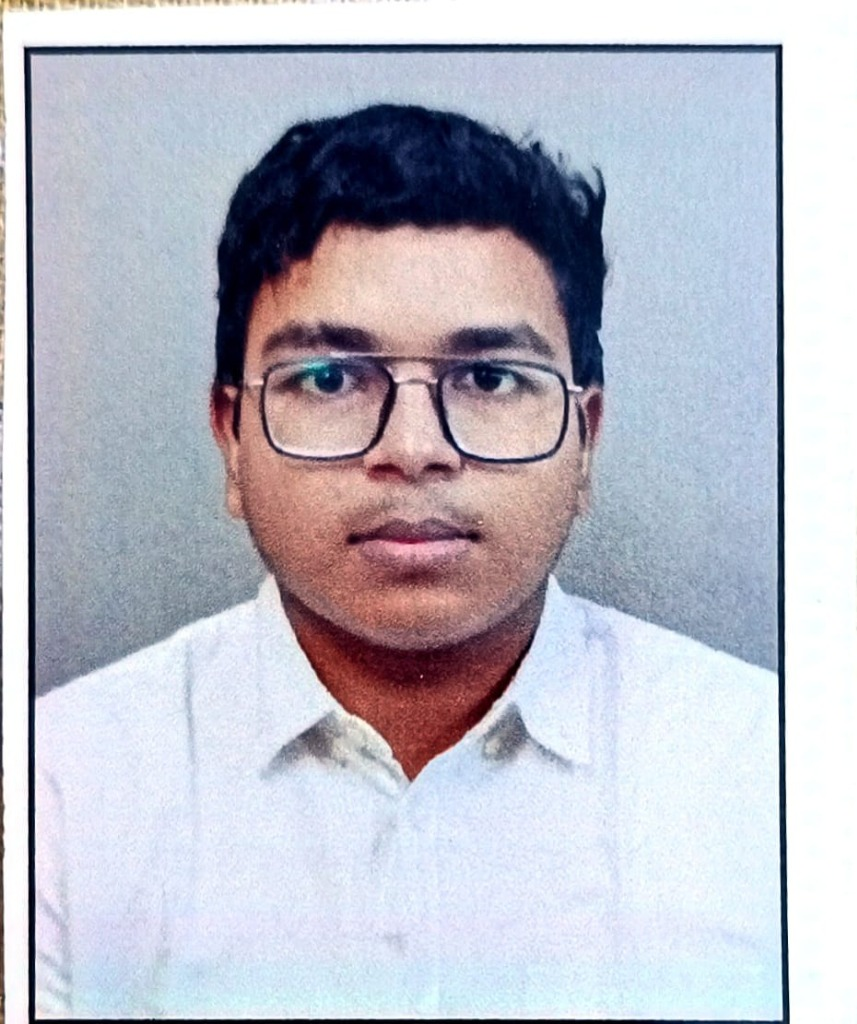
\includegraphics[width=0.82in, height=0.98in, keepaspectratio]{profile.jpg}
\end{minipage}

\vspace{-4pt}

%-----------EDUCATION-----------
\section{Education}
  \resumeSubHeadingListStart
    \resumeSubheading
      {RCC Institute of Information Technology}{Kolkata, West Bengal}
      {B.Tech in Computer Science and Engineering (AIML); CGPA: 8.13/10.0}{Aug. 2023 -- Present}
  \resumeSubHeadingListEnd

%-----------TECHNICAL SKILLS-----------
\section{Technical Skills}
 \begin{itemize}[leftmargin=0.15in, label={}]
    \small{\item{
     \textbf{Core Languages}{: Python, SQL (MySQL, noSQL), Java, JavaScript} \\
     \textbf{AI, ML \& Vision}{: PyTorch, Scikit-Learn, YOLOv8, OpenCV, Fuzzy Logic (Mamdani), Pandas, NumPy} \\
     \textbf{GenAI, RAG \& NLP}{: LangChain, ChromaDB, Transformers (RoBERTa), LLM models, Claude Code, Power BI} \\
     \textbf{Web \& Frameworks}{: FastAPI, React.js, Tailwind CSS, RESTful APIs, Postman API} \\
     \textbf{Tools \& Cloud}{: Docker, Git, GitHub, VS Code, Linux/Bash, Render, Vercel}
    }}
 \end{itemize}

%-----------WORK EXPERIENCE-----------
\section{Experience}
  \resumeSubHeadingListStart

    \resumeSubheading
      {Data Science \& Engineering Intern}{March 2026 -- June 2026}
      {Centre of Excellence on Data Science and Machine Learning}{Kolkata, India}
      \resumeItemListStart
        \resumeItem{Engineered the clinical transcription pipeline for the \textbf{AI Prescription Reader}, integrating \textbf{YOLOv8} for patient PII redaction and \textbf{Gemini Multimodal Vision} to structure EMR data and ICD-10 codes.}
        \resumeItem{Architected a \textbf{Dual-Layer Audit Engine} combining regex rules with \textbf{ChromaDB} formulary vector search; authored and submitted a research paper on the system for the \textbf{National Conference on e-Governance}.}
        \resumeItem{Collaborated across an 18-member engineering cohort to build automated validation scripts, data sanitization routines, and reporting dashboards for unstructured datasets.}
      \resumeItemListEnd

  \resumeSubHeadingListEnd

%-----------PROJECTS-----------
\section{Projects}
    \resumeSubHeadingListStart
      
      \resumeProjectHeading
          {\textbf{AI Prescription Reader \& Dual-Layer Audit Engine} $|$ \emph{FastAPI, YOLOv8, ChromaDB, Gemini Vision, React.js}}{March 2026 -- June 2026}
          \resumeItemListStart
            \resumeItem{Trained a custom YOLOv8 model (91.4\% mAP@50) to dynamically redact sensitive patient PII/signatures and utilized Gemini Multimodal Vision to transcribe handwritten regimens into ICD-10 diagnostic codes.}
            \resumeItem{Built a Vector RAG pipeline using ChromaDB indexing official CMS formularies to phonetically resolve noisy, handwritten drug shorthand with high retrieval accuracy.}
            \resumeItem{Architected a Dual-Layer 100-Point Audit Engine pairing deterministic rule validators with an LLM critic to detect transcript omissions and eliminate clinical hallucinations.}
          \resumeItemListEnd

      \resumeProjectHeading
          {\textbf{FACTCHECK -- Explainable Veracity \& Fake News Intelligence Platform} $|$ \emph{FastAPI, PyTorch, Scikit-Learn, Google News API, Docker}}{}
          \resumeItemListStart
            \resumeItem{Engineered an NLP pipeline on 75K+ articles (WELFake, LIAR, CoAID) with dateline/watermark sanitization; deployed a Dual-Vectorizer linear model (98.7\% accuracy, <5ms CPU latency, <50MB RAM) alongside a PyTorch BiLSTM-Attention model.}
            \resumeItem{Architected a Hybrid Arbitration Engine fusing statistical predictions with live Google News XML wire feeds, Wikipedia refutation cues, claim segmentation, and a 30+ publisher registry to detect mixed-veracity disinformation.}
            \resumeItem{Built an explainability engine with TF-IDF token saliency chips and a 4-tier URL scraper (JSON-LD/DOM); deployed a stateless FastAPI service on Render streaming real-time Veritas Trust Scores (0--100) to a Vercel dashboard.}
          \resumeItemListEnd

      \resumeProjectHeading
          {\textbf{AURA -- Multi-Agent Tutoring System} $|$ \emph{FastAPI, LangGraph, ChromaDB, Gemini 2.5 Flash, React.js}}{}
          \resumeItemListStart
            \resumeItem{Architected a stateful multi-agent tutoring graph via LangGraph and Gemini 2.5 Flash, dynamically routing learners between Socratic hinting, conceptual derivations, and direct remediation.}
            \resumeItem{Engineered a Mamdani Fuzzy Inference System scoring continuous accuracy, latency, and retries into 4 mastery tiers, grounded by an OpenStax ChromaDB RAG store with anti-leak sanitizers.}
            \resumeItem{Developed a full-stack glass-box UI in React.js displaying real-time agent cognitive node activations, state transitions, and timed diagnostic exam analytics.}
          \resumeItemListEnd

    \resumeSubHeadingListEnd

%-----------ACHIEVEMENTS / LEADERSHIP-----------
\section{Achievements \& Extracurriculars}
    \resumeSubHeadingListStart
        \resumeItem{\textbf{Research \& Conferences:} Represented department at National Conference on e-Governance; submitted research paper on clinical prescription auditing.}
        \resumeItem{\textbf{Academic Excellence:} Maintained strong coursework standing with zero backlogs across all semesters.}
    \resumeSubHeadingListEnd

%------------------------------------------- 
\end{document}
